\chapter{実装方法}\label{chap:impl}

前節では,OCaml Blocklyが4つの主な機能をユーザから見た視点で紹介した.
本節では,それぞれについて実装方法を詳細に説明する.本研究はBlocklyに加え\cite{Typed-Blockly}もベースにして行っているため,それぞれの実装も交えて説明を行う.

\section {変数束縛\label{impl:boundVariable}}

まず,Blocklyでの変数ブロックの実装について触れる.
Blocklyでは,新しい変数の追加をフライアウトメニュー内にあるメニューボタンから行う.
既に存在する変数名の追加は行えない.
変数を追加すると,図\ref{fig:blocklyVar}のような変数フィールドを持った数種類のブロックがフライアウトメニューに追加される.
変数フィールドとは,図\ref{fig:blocklyVar}の変数名iを囲う薄いピンク色の部分であり,クリックすると変数名の変更などが行えるブロック内のエレメントである.
各変数フィールドは,内部的に変数インスタンスを保持している.
例えば,図\ref{fig:blocklyVar}に示した3つの変数フィールドは,1つの変数インスタンスを内部的に共有している.
そうすることで,変数名を変更したときに,同じ変数を参照する変数フィールドの変数名が同期的に更新される.
しかし,このBlocklyでの変数の扱いは,関数型言語でのimmutableな変数やシャドウイングをわかりやすく表現するためには相性が悪い.
Blocklyにはスコープという概念がなく,全ての変数はグローバルな変数として扱われているため,同名の複数の変数を扱うことができないためである.

\begin{figure}[h]
 \centering
 \vspace{-1.0zh}
 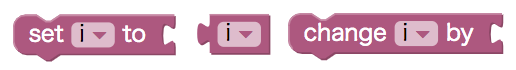
\includegraphics[keepaspectratio, scale=0.3]{img/iVar.png}
 \caption{本来のBlocklyにて,ブロック内に変数フィールドを持つ3つのブロックの例.\label{fig:blocklyVar}}
\end{figure}

束縛変数とその束縛関係を表現するには,変数インスタンスの種類を「宣言される変数」と「宣言される変数を参照する変数」に分けると都合がよい.
参照する変数は,自身がどの変数を参照しているのかを保持し,変数名を取得したいときや変更したいときはそれに問い合わせれば,変数名が変更されたときの各変数フィールドの更新を元のBlocklyと同様にシンプルに行うことができる.

実装の詳細を説明する.
1つの変数は,1つの束縛変数宣言と,0個以上の変数参照と関連付けられる.
この変数宣言と変数参照を表現するため,以下の2つのクラスを定義した.

\begin{description}
 \item[{\tt BoundVariableValue}] 束縛する変数,宣言される変数.
 \item[{\tt BoundVariableValueReference}] 束縛される変数,宣言された変数を参照する変数.
\end{description}
Blockly の変数フィールドは束縛変数フィールドに拡張され,それぞれの束縛変数フィールドは,それが変数宣言であるか変数参照であるかによって,2つのうちどちらかのクラスのインスタンスを持つ.

これらのクラスを用いて,スコープチェックを以下のように実装した.
変数宣言を持つブロックは,スコープを作るコネクタを引数として,スコープ内で参照できる変数の一覧を返す関数を定義する.
この関数を用いて変数環境を更新して,スコープ内のブロックに存在する全ての変数参照が変数環境にあるかどうかを調べれば良い.
この作業を再帰的に行えば,ネストしたブロック全体のスコープチェックが行える.
ユーザがある 2 つのコネクタを接続しようとしたときは,接続を仮定したスコープチェックを行い,失敗した場合は接続を拒絶する.

次に,束縛変数フィールドの描画について説明する.
変数宣言か変数参照かどうかによって束縛変数フィールドの描画の仕方を変える.
変数宣言の場合は,ブロックの形を模したSVGを背景に描画し,変数宣言部分から変数ブロックの生成を行えることを表現する.
そして,実際にドラッグされたときにその変数への参照を持つブロックを生成する.
束縛変数フィールドをホバーしたときに,関連した全ての変数フィールドをハイライトする機能は,変数宣言が自身を参照する変数の一覧を保持することによって行える.
変数宣言に問い合わせて関連した全ての変数を取得したら,それら変数を内包する各フィールドの背景色を変える.

\section {スコープお砂場\label{impl:osunaba}}

スコープお砂場のようなメインワークスペースとは独立した作業空間を実現するには,まずワークスペースをもう1つ作ればよい.
そうすることによって,メインワークスペースとは分離した別のブロックを組み立てる世界を作ることができる.

スコープお砂場内でのスコープチェックはメインワークスペースとは異なる.
メインワークスペースでのスコープは空の変数環境であるが,お砂場でのスコープは所属先のスコープで使える変数を全て含んだ変数環境である.
このお砂場が持つスコープは,お砂場を所有するブロックを上位から辿っていくことにより取得する.
これは,構文木を上から辿って変数環境を更新していくインタプリタと似た要領である.
お砂場が入れ子になっている場合は,親のお砂場が持つスコープも同様に取得する.
ユーザがブロックをお砂場の上にドラッグしてきたときには,移動中のブロック内の自由変数が全てお砂場のスコープで有効かを調べる.
そうでない場合は,お砂場内で参照できない変数を含んでいるときなので,ブロックのお砂場への移動を拒絶する.

また,スコープから参照できる変数ブロックを並べたフライアウトメニューをお砂場に実装した.これによって,ユーザはお砂場内で使用できる変数の一覧を知ることができ,また,変数参照ブロックの生成も直接そこから行うことができる.
スコープお砂場を所有するブロックの移動によって,お砂場の暗黙的な変数環境が変わるときは,即時的にフライアウトメニューを更新する.

お砂場にブロックを持ちよって自由に組み立たり,その後に別のワークスペース内のブロックと接続させたりするには,ブロックが異なるワークスペース間を移動できるようにする必要がある.
本来のBlocklyでは,ブロックの自由な組み立てはメインワークスペースでしか行われないため,ワークスペースを越えたブロックの移動は想定されていない.
このため,本システムではブロックのワークスペース間の移動を実装した.実装の方法は主に2つあると考えられる.

1つの方法はブロックのSVGを移動先のワークスペースのSVGグループに移動させ,ブロックオブジェクト内の古いワークスペースへの参照を全て更新することである.%先行研究は過去形に????
この方法はあまり現実的でない.
なぜならワークスペースと繋がりを持つのはブロックのみでなく,コネクタやフィールドなどといったブロック上に存在する不特定多数のコンポーネントも,ワークスペースを参照し合ったり,イベントリスナーを登録したりするなどしてワークスペースに依存しているためである.それら全てのワークスペースへの依存を完全に正しく更新するのは煩雑であり,将来の拡張のたびに変更が必要な,技術的負債となりうる.
%BlocklyをベースにすることでUIの実装を省いているため,Blocklyの実装を安全に利用したい.

もう 1 つの方法は移動先に新しいブロックを作り直し,古いブロックを削除することである.
この方法は, Blockly に元々あるブロックのエンコード,デコード機能をうまく使うことによって,比較的容易に確実な実装をすることができる.

\subsection*{XMLを利用したブロックの再構築}

Blockly では,ブロックをXML にエンコード,XMLからブロックにデコードできるようになっている.
このブロックとXMLの双方向の変換は,従来のBlocklyにていろいろな場面で活用されている.
例えば,デモページを作るとき,フライアウトメニューにどの種類のブロックを備えるかはXMLで指定することになっている.
指定するXMLを入れ子にすれば,接続した複数のブロックをフライアウトメニュー上に並べることもできる.
%例えば,フライアウトメニューからブロックを生成する際には,元型のブロックをXMLにし,メインのワークスペースにてXMLに従ってブロックを作り上げることによって行なっている.

本研究では,このブロックとXMLの双方向変換を利用して,ワークスペース移動時のブロックの再構築を行なった.
移動したいブロックを XML にエンコードし,その XML から新しいブロックをデコードして得る.
このとき,気をつけるべきことが2つある.
1つはブロック内の変数の参照関係が新しいブロックでも保たれていること,もう1つは古いブロックにあった全ての型表現を新しいブロックへと移し替えることである.

まず,作り変えの後も変数の参照関係を保つために,エンコード時にはブロック内の変数参照がどの変数を参照していたかという情報もXMLに落とす必要がある.
この変数の参照関係のエンコードは,自由変数であるものに対してのみ行う.
そうでないと,新しいブロック上の変数が古いブロック上にある変数を参照してしまうことになり,それはワークスペース間の移動後に削除されてしまうからである.
エンコードされなかった変数の参照関係は,ブロックを組み立て終えたのちに,各スコープの変数環境に従って自動で復元する.

次に必要なことは古いブロックにあった型表現を全て新しいブロックの同じ位置のコネクタに移し替えることである.
これは型変数の固有の色をブロックの作り直しの前と同じ色に保つためであり,型表現の移し替えを行うことで,ブロック上の型変数が既に何か具体的な型に単一化されていたとしても,接続を解除したときに元の色に戻れるようにすることができる.

なお,XMLをデコードして新しいブロックを組み立て直す最中はブロックに対するスコープチェックを無効にする.
ブロックは深さ優先で組み立てられていくが,例えば「{\tt let x = ... in x + 42}」の足し算ブロック部分「{\tt x + 42}」を組み立てる最中に,xがスコープにない変数になってしまうからである.また,ブロックに付属したスコープお砂場も同様に新しいブロックへと移動させるが,その説明はここでは割愛する.
% let f = f + x を let x = d + d in 

\section {let多相を含んだ型システム\label{katasuiron}}

Blocklyは型を文字列による名前で表現することによって,簡単な型チェックをサポートしている.各コネクタに型の名前を保存することができ,型が設定されている場合は,同じ名前の型を持つコネクタとしか接続できないようにすることで,単純な型付けを行なっている.

型を文字列で区別してしまうとList型などのパラメタ付き型を表現することは難しいが,
\cite{Typed-Blockly}では各コネクタに文字列の代わりに型変数などの型表現を加えることによってパラメタ付き型をブロック上に実装している.
型の単一化が可能な型表現を持つコネクタ同士でしか接続できないようにし,接続する際には2つのコネクタが持つ型表現を単一化する.
一方で,\cite{Typed-Blockly}では連結させたブロックを外したとき型の単一化が解除されないことや,構文に沿った型推論,let多相が実装されていないなど,拡張が必要な部分がある.

\subsection*{型の単一化の解除}
ユーザがブロックを外した際に型の単一化の解除を行うには,コネクタに添付した型変数の単一化の関係を全て削除したのち,構文の意味に沿ってもう一度型推論を走らせることが必要である.
新しい型変数を振り直すことも単一化解除の1つの方法だが,本システムでは型変数を固有の色で表現しており,解除後にも同じ色を保つ必要があるため,型変数の振り直しは行わない.
型付きブロックのクラス定義それぞれに,以下の2つインスタンス関数を定義する.
\begin{description}
 \item[{\tt clearTypes()}] ブロックに存在する全ての型変数の単一化の関係を削除する.
 \item[{\tt inferTypes(env)}] ブロックの構文に沿って型推論を行う.
引数{\tt env}は型環境であり,変数名をキーとして型スキームを値として持つオブジェクト.返り値としてブロックの出力の型を返す.
\end{description}

ある2つのブロックの接続が外れたとき,全ブロックのトップのブロックから{\tt clearTypes},{\tt inferTypes}を順に実行すればよい.

\subsection*{let多相の実装} %letたそうの説明加える?
let多相を実装するには,ブロックの接続解除時だけでなく,接続時にもトップのブロックから型推論を実行する必要がある.
値制限を設けているためブロックの付け替えによって単相,多相との切り替えが起こりうるためである.
また,スコープお砂場にあるブロックにも型推論を行うことを考えると,型推論を行うブロックの順番も重要である.
束縛型変数を持つ型スキームの場合,letで宣言した変数の型スキームの解決は,必ずスコープお砂場にあるブロックに型推論を走らせるよりも前に行わなくてはならない.
スコープお砂場にletで宣言した変数に束縛された変数ブロックに型推論を走らせるとき,その型スキームが必要になるからである.
% https://developers.google.com/blockly/guides/create-custom-blocks/type-checks

\section {メッセージ出力}

第\ref{sec:honkenkyu}節で述べた通り,本研究で防ぐ対象とするエラーは,シンタックスエラー,型エラー,Unbound valueエラーの3つである.
シンタックスエラーはブロック上では起き得ないとして,ドラック中のメッセージ出力は型エラー,Unbound valueエラーの2つに対して行うとする.

ユーザになぜ期待通りの動作が行えないのかを説明するべきシーンは,以下の2つがある.
\begin {itemize}
  \item 接続してしまうと型エラーあるいはUnbound valueエラーが起きてしまうコネクタ同士を繋げようとしたとき.
  \item 変数を含んだブロックを変数環境に正しく束縛されず,Unbound valueエラーが起きてしまう場所にドラッグしたとき.例えば,「{\tt x; let x = 5}」など.
\end {itemize}

1つ目におけるエラーを取得するためには,接続可能なコネクタを探索する処理を拡張する.
元のBlocklyには,近傍にあるコネクタの中から接続可能なものを探す処理がある.
この接続可能かどうかの判断はOCaml Blocklyのために拡張されたため,第\ref{impl:boundVariable}節で触れたようなスコープチェックや,型チェックが含まれている.
近くのコネクタが全て接続可能でない場合,最も近いコネクタに対するエラーメッセージをツールチップに表示する.
このエラーメッセージは,Unbound valueエラー,型エラーに関する詳細をユーザに通知する.

2つ目は,ブロックを接続させずに移動させる動作になる,すなわち,十分に近いコネクタが存在しない場合である.この場合は,ドラックされているブロックに対してスコープチェックを行い,正しく変数環境に束縛されない変数が存在するならば,そのエラーメッセージを取得し,表示すればよい.


